\documentclass{thesis}

% User defined colors
\definecolor{LightPink}{HTML}{F7EFF7}
\definecolor{Wisteria}{HTML}{C3AFDD}
\definecolor{Petrol}{HTML}{12939A}
\definecolor{Honeydew}{HTML}{E8FFE0}
\definecolor{DarkSeaGreen}{HTML}{80B192}
\definecolor{MarkStroke}{HTML}{4b4e6d}
\definecolor{MarkFill}{HTML}{8487aa}

\hypersetup{
  unicode=true,
  pdftitle={English MSc Thesis Template},
  pdfauthor={Panayiotis I. Vlantis},
  pdfsubject={Big Data},
  pdfkeywords={Big Data,latex,thesis,template},
  pagebackref=true,
  colorlinks=true,
  linkcolor=black,
  citecolor=black,
  urlcolor=black
}

\begin{document}

\title{
  MsC Thesis Template
}{
  Πρότυπο για Διπλωματικές Εργασίες
}

\header{MSc Thesis Template}

\date {July 2018}
      {Ιούλιος 2018}
      {Ιουλιος 2018} % Greek without accent

\author {Panayiotis I. Vlantis}
        {Παναγιώτης Ι. Βλαντής}{M1387}
        {P. Vlantis}

\supervisor {Alex Delis}{Professor}
            {Αλέξης Δελής}{Καθηγητής}

\commitee  {Alex Delis}{Professor}
           {Αλέξης Δελής}{Καθηγητής}
           {Maria Roussou}{Assistant Professor}
           {Μαρία Ρούσσου}{Επίκουρη Καθηγήτρια}

\subject {Big Data}{Δεδομένα Υψηλής Κλίμακας}

\keywords {
  big data,
  latex,
  thesis,
  template
}{
  δεδομένα υψηλής κλίμακας,
  πρότυπο,
  διπλωματική
}

\abstract {
  English Abstract...\\ \blindtext
}{
  Περίληψη στα Ελληνικά....\\ \blindtext
}


\maketitle

\begingroup
  \hypersetup{linkcolor=black}
  \tableofcontents
  \thispagestyle{empty}
  \clearpage
  \listoftables
  \thispagestyle{empty}
  \clearpage
  \listoffigures
  \thispagestyle{empty}
  \clearpage
\endgroup

\chapter{Introduction}

\section{How to do some things}

\subsection{How to work with figures}

I use Inkscape\cite{inkscape} to create figures in SVG format.
I prefer working with SVG images but I would like to use their EPS version
in the latex document.
I achieve that by saving the SVG image in the figures directory and generate
the EPS version using inkscape from command line.
\fbox{\footnotesize{\texttt{
  inkscape --export-eps=figures/build/myimage.eps figures/myimage.svg
}}}

\begin{figure}[h!]
  \centering
  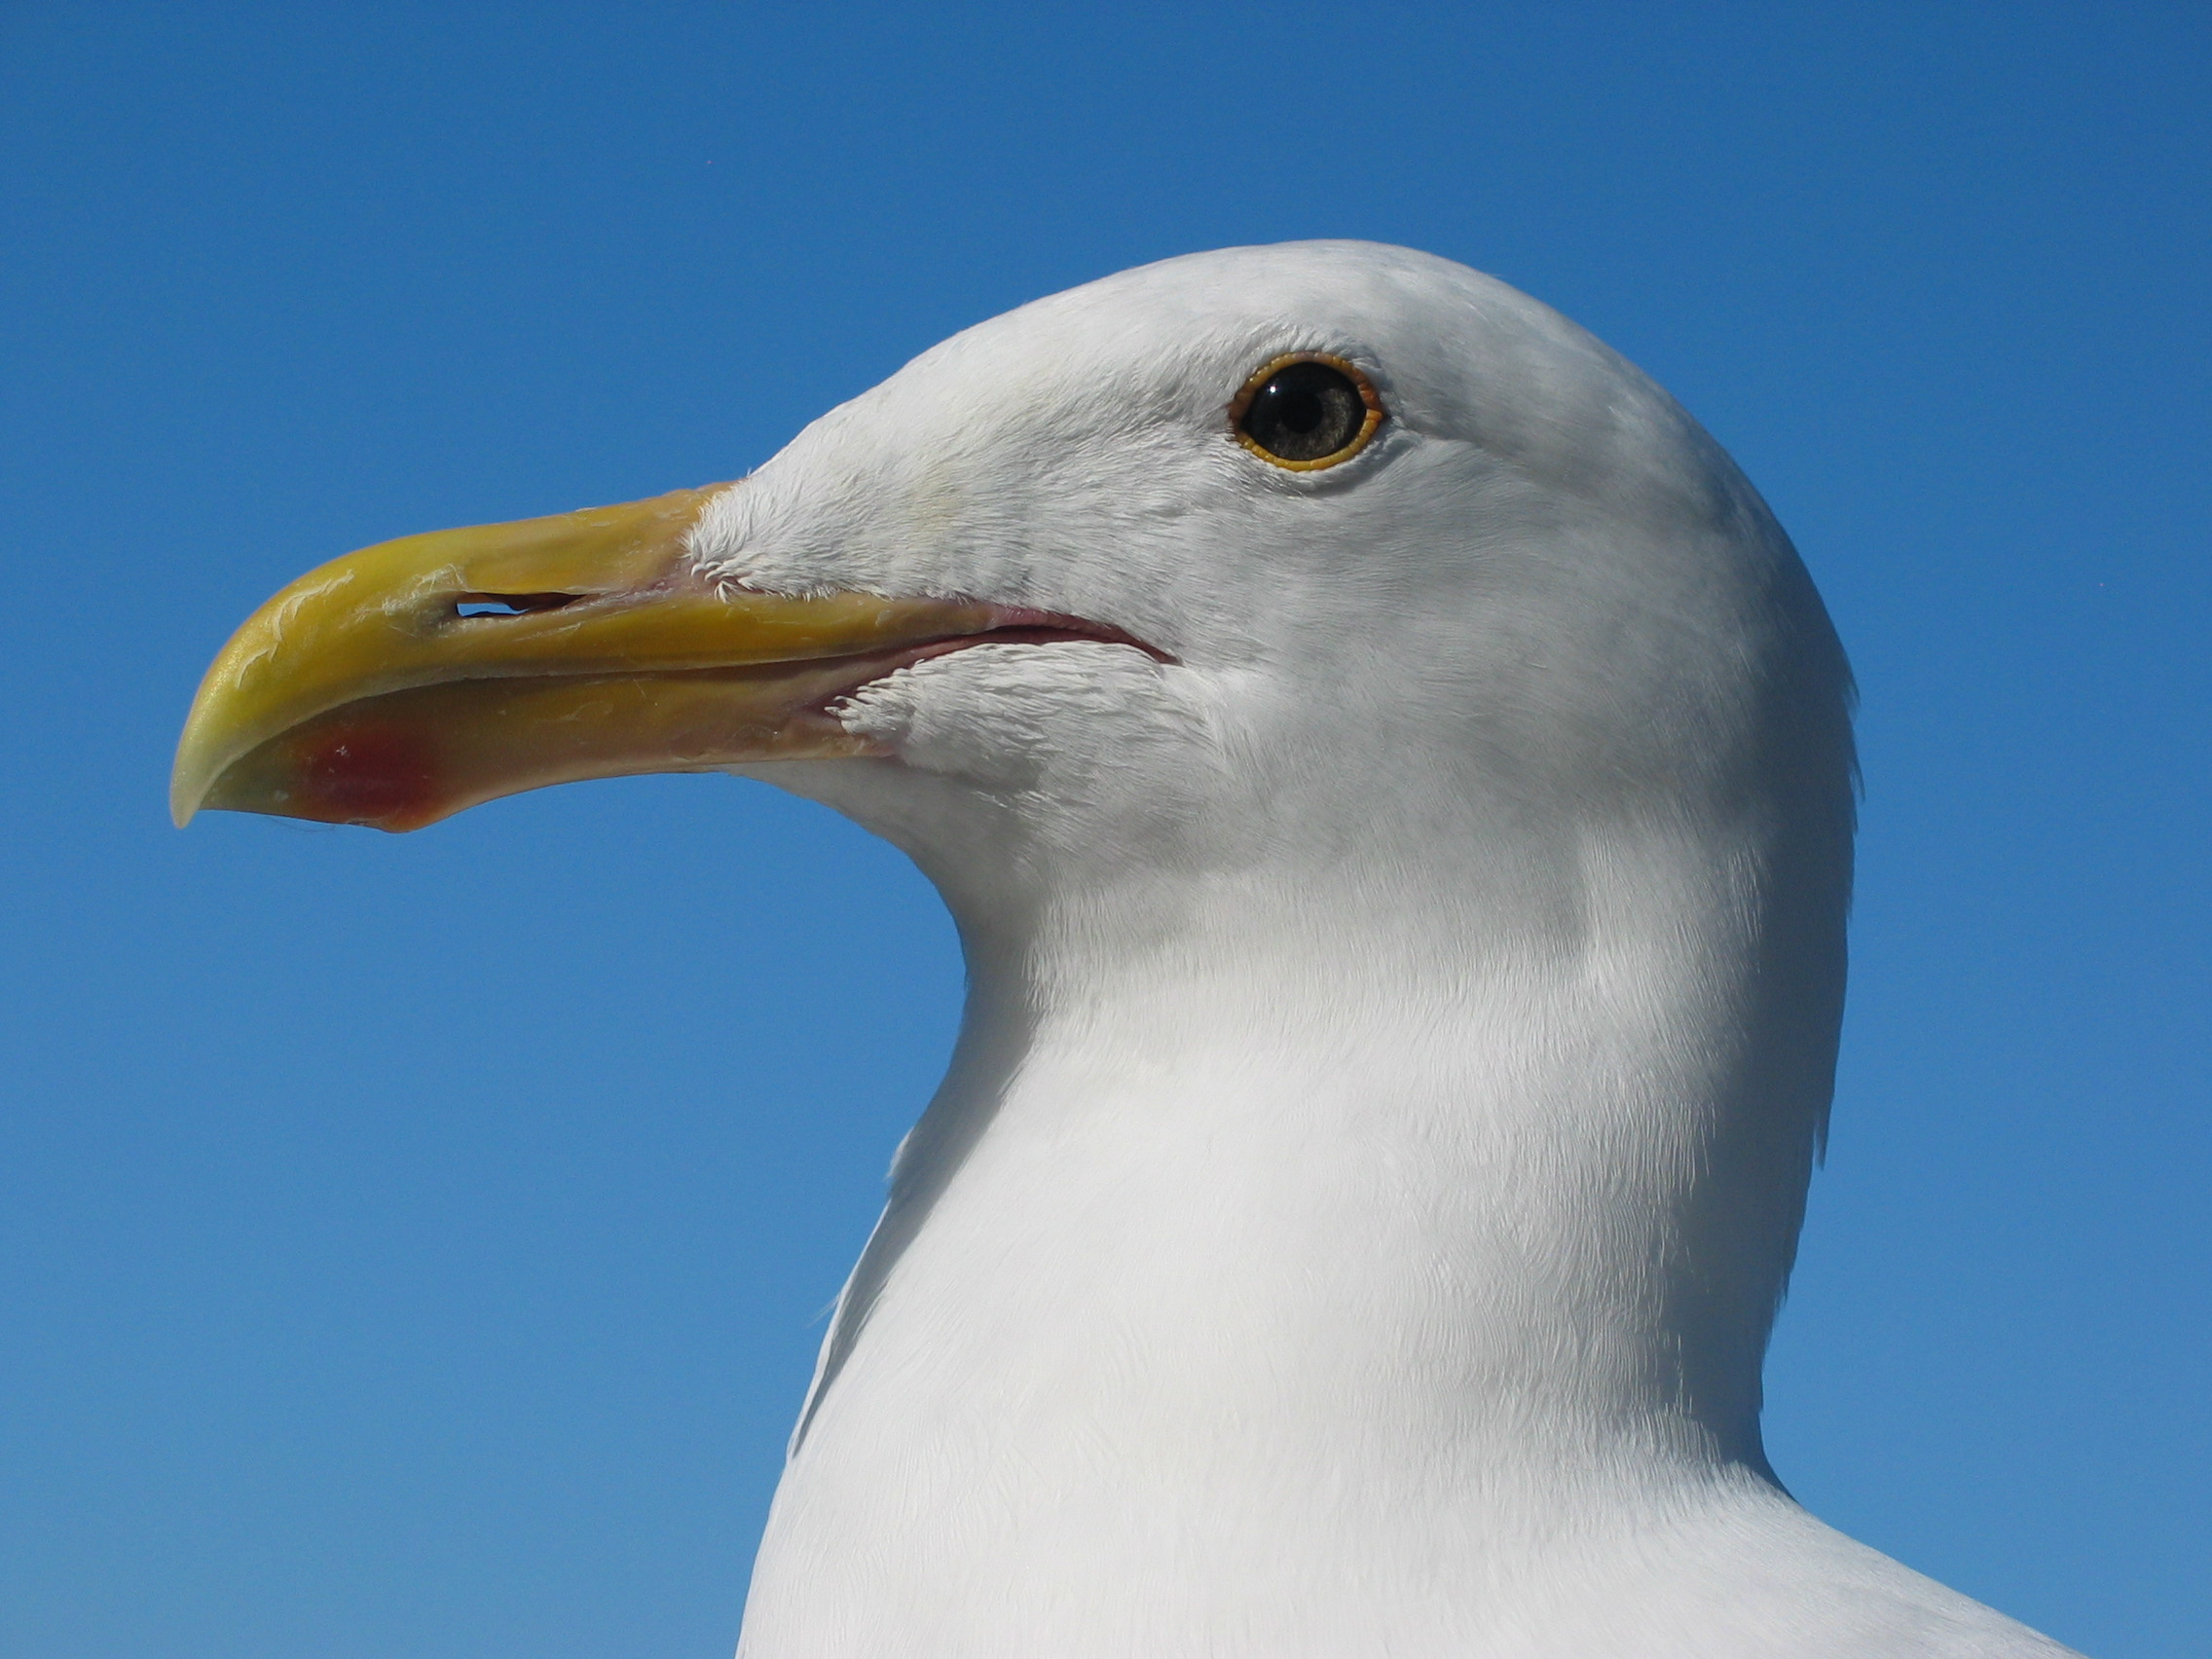
\includegraphics[width=0.6\textwidth]{gull}
  \caption[Example gull photo]{
    This photograph of a gull was the first Quality
    image to be promoted to Featured Pictures status
    in Wikidedia Commons.
  }
  \label{fig:gull}
\end{figure}

\todo[inline]{
  Package todonotes provides inline notes like this.
}
To add file figures/gull.png as a figure:

\begin{minted}[xleftmargin=10pt,fontsize=\footnotesize]{tex}
  \begin{figure}[h!]
    \centering
    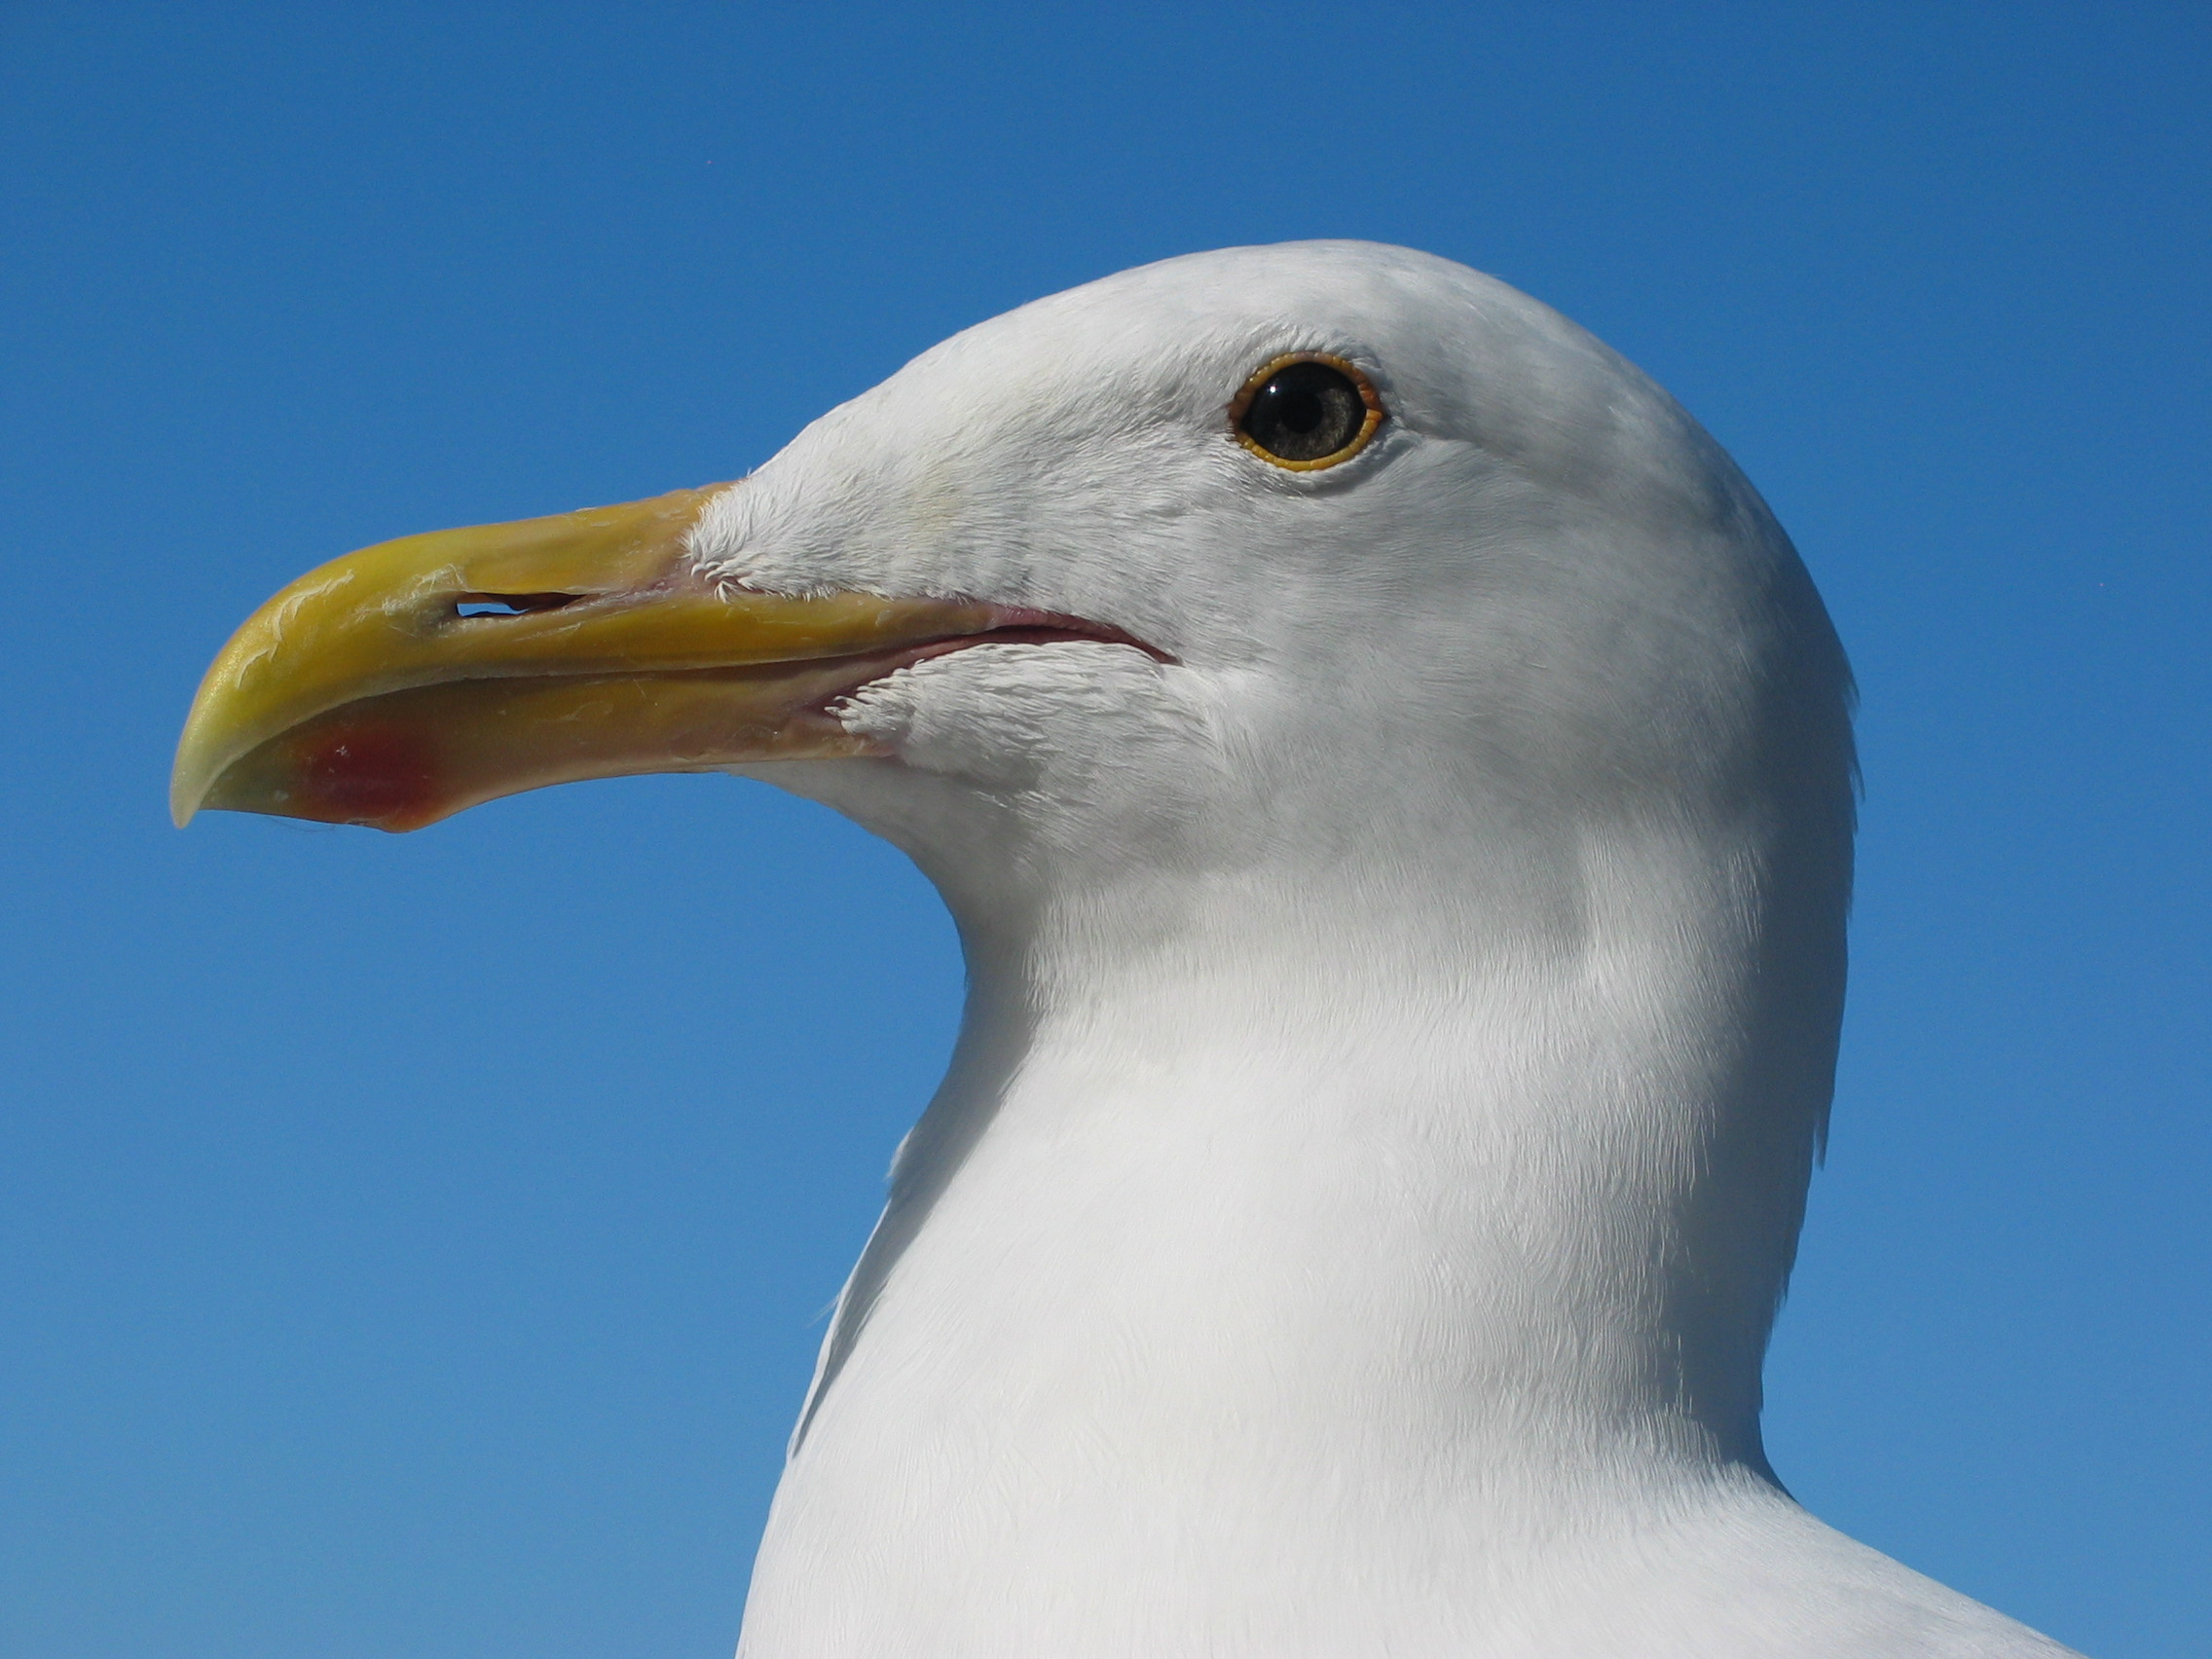
\includegraphics[width=0.6\textwidth]{gull}
    \caption[Example gull photo]{
      This photograph of a gull was the first Quality
      image to be promoted to Featured Pictures status
      in Wikidedia Commons.
    }
    \label{fig:gull}
  \end{figure}
\end{minted}

\subsection{How to add a table with caption on top}

Tables are a common feature in academic writing, often used to summarize
research results. Mastering the art of table construction in LaTeX is therefore
necessary to produce quality papers and with sufficient practice one can print
beautiful tables of any kind. \cite{latextables}

\begin{table}[h!]
  \centering
  \caption[Example table with caption on top (List of Tables caption)]{
    Notice how the table's caption is on top of the table and centered.
  }
  \begin{tabular}{| p{25mm} | p{20mm} | p{20mm} | p{80mm} |}
    \hline
    Day & Min Temp & Max Temp & Summary \\
    \hline
    Monday & 11C & 22C & A clear day with lots of sunshine.
    However, the strong breeze will bring down the temperatures. \\
    \hline
    Tuesday & 9C & 19C & Cloudy with rain, across many northern regions.
    Clear spells across most of Scotland and Northern Ireland,
    but rain reaching the far northwest. \\
    \hline
    Wednesday & 10C & 21C & Rain will still linger for the morning.
    Conditions will improve by early afternoon and continue
    throughout the evening. \\
    \hline
    \end{tabular}
\end{table}

\begin{minted}[xleftmargin=10pt,fontsize=\footnotesize]{tex}
  \begin{table}[h!]
    \centering
    \caption[Example table with caption on top (List of Tables caption)]{
      Notice how the table's caption is on top of the table and centered.
    }
    \begin{tabular}{| p{25mm} | p{20mm} | p{20mm} | p{80mm} |}
      \hline
      Day & Min Temp & Max Temp & Summary \\
      \hline
      Monday & 11C & 22C & A clear day... \\
      \hline
      Tuesday & 9C & 19C & Cloudy with rain... \\
      \hline
      Wednesday & 10C & 21C & Rain will still... \\
      \hline
      \end{tabular}
  \end{table}
\end{minted}

\subsection{How to add a plot}
PGFPlots draws high-quality function plots.
The user supplies axis labels, legend entries and the plot coordinates for
one or more plots and PGFPlots applies axis scaling, computes any logarithms
and axis ticks and draws the plots, supporting line plots, scatter plots,
piece­wise constant plots, bar plots, area plots, mesh and surface plots and
some more \cite{pgfplots}.
%
Examples of PGFPlots are available in
\href{http://pgfplots.sourceforge.net/gallery.html}
     {pgfplots.sourceforge.net/gallery.html}

\begin{figure}
  \centering
  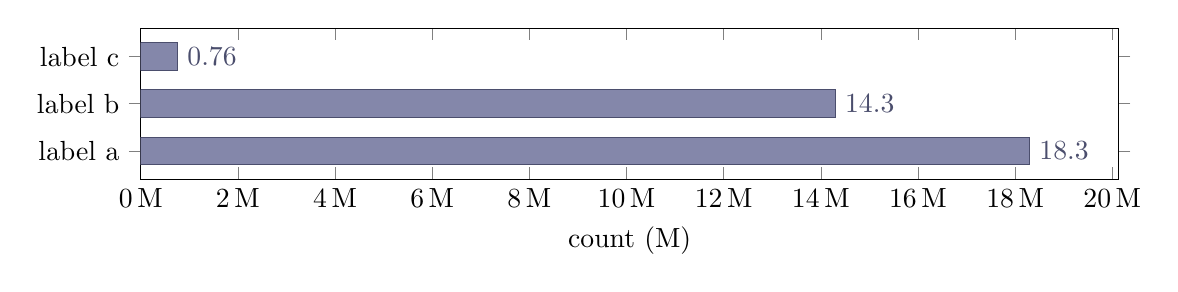
\begin{tikzpicture}
    \begin{axis}[
      xbar, xmin=0,
      width=14cm, height=3.5cm,
      enlarge y limits=0.3,
      xlabel={count (M)},
      symbolic y coords={label a,label b,label c},
      ytick=data,
      nodes near coords, nodes near coords align={horizontal},
      xticklabel = \pgfmathprintnumber{\tick}\,M
    ]
      \addplot[MarkStroke,fill=MarkFill] coordinates {
        (18.3,label a)
        (14.3,label b)
        (0.76,label c)
      };
    \end{axis}
  \end{tikzpicture}
  \caption[Horizontal plot with custom colors]{
    This is a horizontal plot with custom colors.
    More examples are available in\\
    \href{http://pgfplots.sourceforge.net/gallery.html}
         {pgfplots.sourceforge.net/gallery.html}
  }
  \label{fig:plot-2}
\end{figure}

\section{How to build the pdf}

\texttt{Latexmk} is used to build the pdf instead of
calling \texttt{xelatex} directly.
%
\texttt{Latexmk} is a perl script for running LaTeX
\emph{the correct number of times} to resolve cross references, etc;
it also runs auxiliary programs like bibtex.
%
Checkout the manual of Latexmk:
\href{http://mg.readthedocs.io/latexmk.html}{mg.readthedocs.io/latexmk.html}.
%
Its configuration resides in the localfile \texttt{.latexmkrc}.
%
There is also a \texttt{Makefile} but it is a wrapper around \texttt{Latexmk}.
%
So either running \fbox{\footnotesize{\texttt{make all}}}
or \fbox{\footnotesize{\texttt{latexmk}}}
builds the pdf.



\begin{appendix}
  \addcontentsline{toc}{chapter}{APPENDICES}
  \appendixstartedtrue
  \chapter{Thesis Class File}

Minted package is used for code highlighting

\inputminted[fontsize=\scriptsize,linenos]{tex}{thesis.cls}

\end{appendix}

\hypersetup{linkcolor=black}

\bibliography{library}{}
\bibliographystyle{IEEEtran}
\end{document}
